\chapter{Implementation internals}
\addtocontents{toc}{\protect\setcounter{tocdepth}{0}}
\label{app:implementation}

This section provides insights on the code from a programmer's point of view. We do not focus on algorithms here, as we already did that in \cref{chapt:Implementation}. The main focus here is on data representation and division of code into multiple modules.

\section{Design and Libraries}
Logically, the program consists of four components, and they are Physics, Graphics, Mesh Manipulation and Controllers. Controllers connect the other three components together, see~\cref{fig:architecture}. In the following list, we explain the purpose and summarise used technology in each of them.
\begin{description}
\item[Physics] provides us with the simulation of our objects and collision detection. We use \emph{Bullet physics} to implement this component.
\todo{ref na bullet do 2.}
\item[Graphics] is used for rendering the current state of the physics world. Although it is possible directly use those low-level libraries, we use a library with more abstraction in provided API. Using higher-level libraries means we can save code, but we lose a direct control of rendering process. This thesis is not focused on graphical output and only uses it as a tool for building our application.

We decided to use \textbf{Irrlicht Engine}~\footnote{\url{http://irrlicht.sourceforge.net/}}. Irrlicht is a light-weight cross-platform, high-performance engine capable of using either  \emph{OpelnGL} or \emph{DirectX}. Our use of Irrlicht is based on using its graphical window as an output of our application and also using Irrlichts event receiver for reading user input.

\item[Controllers] ask the Physics to step the simulation and provided collision data and give the information about the current state of the world to the Graphics. The Controllers also read the user input which is done by parts of \emph{Irrlicht engine}. Mesh Manipulation component is called to create new objects and react to the collision provided by the Physics.
\item[Mesh Manipulation] provides tools for creating objects, creating a Voronoi cell (done by \emph{Voro++}, converting data and handling the collisions. To be able to do the mentioned tasks, Mesh Manipulation works closely with \emph{CGAL} library and also use \emph{HACD} library for convex decomposition.
\end{description}



\section{Data representation}
As a result of using multiple libraries for a multitude of tasks, we have to deal with a lot of different data representations of the same objects. 

We introduce the data structures that are used to represent one in-game object for multiple purposes. We can see how different data types are converted in~\cref{fig:conversions}.

\begin{figure}
        \centering
        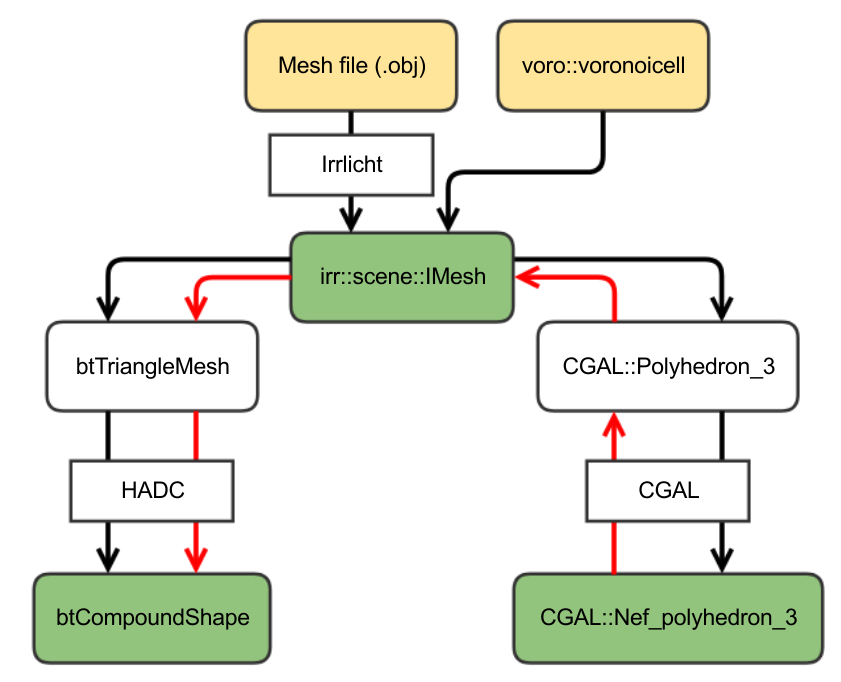
\includegraphics[width=\textwidth]{img/conversions}
        \caption{Data conversion diagram. Input formats - yellow, required formats - green. Black lines show used conversions, red lines show required process after a change of the shape of an object. Rectangles signify the library used to make the conversion, if none a member function of {\tt gg::MMeshManipulators} is used.}
        \label{fig:conversions}
\end{figure}

\subsection*{\tt btRigidBody}
\emph{Bullet physics} uses this class to hold information about a rigid collision object. For us, most important part of the body is a collision shape.

The collision shape can be of multiple types, most notably a convex hull or a primitive geometric shape, a triangular mesh or a compound shape. We need the collision shape to be as close to a visual mesh as possible. Because calculating collision between triangular meshes is not implemented in the \emph{Bullet physics} and would be too costly even if implemented, we choose the representation by compound shape.

One more parameter of {\tt btRigidBody} to consider is the object mass. Bodies with mass set to zero (or negative value) are considered static objects and do not move. Bodies with positive mass react to gravity and other external forces, their centre of gravity is set to their respective origin of local coordinates. This poses a problem when the origin is not inside the object. 

We try to solve the problem of displaced origin by calculating a centre of the bounding box of the object and then translating all vertices in a way that the centre becomes an origin. After the origin is changed, we must appropriately adjust the position of the object. We deployed this approach to newly created objects. The difference between where the real centre of gravity should be, and where the centre of gravity used by Bullet physics is, is not visible. However, we failed to solve this problem with objects with their mesh changed. This results in the visibly displaced centre of gravity and occasional wrong position of newly created objects. Because this problem has no impact on the simulation of the destructible environment, we decided against trying to solve it.

\subsection*{\tt irr::scene::ISceneNode} 
Graphical object in the \emph{Irrlicht engine} is represented by this class. It is an abstract class instantiated into multiple types of graphical objects, \eg lights, cameras, animations, particle systems. To represent our objects, we are using {\tt irr::scene::IMeshSceneNode}. {\tt irr::scene::IMesh} is the data structure inside {\tt irr::scene::IMeshSceneNode} that stores the mesh information. 

\subsection*{\tt irr::scene::IMesh} 
This class stores the mesh information in multiple mesh buffers. Each buffer has an array of vertices and an array of indices. Every index in the array of indices refers to one vertex. However, we found out that not every vertex is referred to, and therefore valid. Indices divided into consecutive non-intersecting triples form a triangular face of a mesh. 

\subsection*{\tt CGAL::Nef\_polyhedron\_3}
\label{sec:nef}
"A Nef-poly-he-dron in dimension $d$ is a point set $P \subseteq \mathbb{R}^d$ generated from a finite number of open halfspaces by set complement and set intersection operations."~\footnote{\url{http://doc.cgal.org/latest/Nef\_3/index.html\#Nef\_3Definition}} In other words, {\tt CGAL::Nef\_polyhedron\_3} is a boundary represented data structure closed under Boolean operations. This make it ideal to perform our boolean operation on.
This structure imposes a restriction on the data we can use to represent our objects, the underlying halfedge data structure~\footnote{\url{doc.cgal.org/latest/HalfedgeDS/index.html\#Chapter\_Halfedge\_Data\_Structures}} is restricted to orientable 2-manifolds. Common examples of non-manifold geometry: open geometry, two neighbouring faces with opposite normals, two faces sharing vertex but no edge, self-intersecting geometry, inside faces.

\subsection*{\tt gg::MObject} 
{\tt gg::MObject} is a class designed to unite all data about one in-game object into one structure. It includes {\tt irr::scene::ISceneNode}, {\tt btRigidBody} and {\tt CGAL::Nef\_polyhedron\_3}. It implements the mechanism ensuring that upon deletion of an object, its parts are first removed from their respective engines, and then safely deallocated before {\tt gg::MObject} itself is destroyed.


\section{Modules}
In this section, we describe the functionality of each program module. Third party software is not be described here, details about used libraries can be found in \cref{chapt:technology}. Interactions between modules are visualised in \cref{fig:modules}. \emph{Irrlicht Engine} is not present in the diagram because we do not structurally depend on it. Every module is contained in a file of the same name, as a class with that name prefixed with letter M (\ie Object Creator can be found in file ObjectCreator.cpp and is implemented as class {\tt gg::MObjectCreator}). Also, namespace {\tt gg} identifies exact components of the application implemented for this thesis.

\begin{figure}
        \centering
        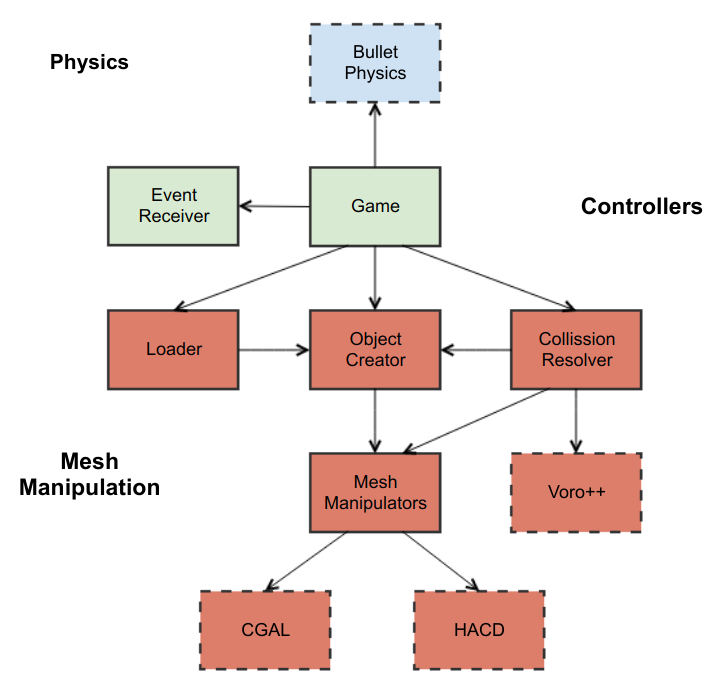
\includegraphics[width=\textwidth]{img/objectmodel}
        \caption{Software architecture shown on diagram of relationships of program modules. Third party software is highlighted in dashed rectangles.}
        \label{fig:modules}
\end{figure}

\begin{description}

\item[Game] module holds {\tt gg::MGame} class which is the core of the application. The communication with the physics engine,  the graphical engine and mesh manipulation parts of the software is managed from here.

\item[Event Receiver] module implements the instance of {\tt irr::IEventReceiver} from Irrlicht engine and it is used to read the user input.

\item[Loader] is only used for initializing the application. It parses the data that describe the game environment from the \emph{medial/world.cfg} file, constructs the objects using {\tt gg::MObjectCreator}, and returns the set of constructed objects.

\item[Object Creator] implements the {\tt gg::MObjectCreator} class designed in a Builder pattern to provide initialization for the data contained inside {\tt gg::MObject}.

There are three member functions that allow us to create {\tt gg::MObject}s  with different behaviours from the same set of input parameters (see \cref{sec:data}). We can create a destructible object, an indestructible object with box collision shape and a rectangular indestructible object without input mesh.  Those functions are meant to be used exclusively for application initialization, as they generate a new convex decomposition and {\tt CGAL::Nef\_polyhedron\_3} from their mesh.

Two more kinds of objects can be created: a projectile that is shot from the given position with the given impulse and a destructible object with temporary collision shape (sphere shaped). Because the object with temporary collision shape is constructed while the game is being played and construction of {\tt CGAL::Nef\_polyhedron\_3} can take a longer time, to gain controll over the construction, we will construct it beforehand and then provide it to the Object Creator.

\item[Collision Resolver] implements the Collision handling process, described in~\cref{sec:collisions}. Conversions between data formats that are required during the process are externalised to Mesh Manipulators module to maintain the code readable.

\item[Mesh Manipulators] provides set of utility functions. Because different libraries are used for physics simulation, rendering and geometric manipulation, those functions provide means for converting data between different formats.
\end{description}

